\chapter{Estudio del Problema}

\section{Definiciones, Siglas y Abreviaciones}
Como aclaración inicial, \textbf{Re-Volt America} es un nombre propio de comunidad, el cual se escribe sin acentuar la letra ''e'' como vendría normalmente acentuada en el idioma español. El anglicismo de ''America'' es completamente intencional, ya que el nombre proviene del idioma inglés americano.

A continuación, se definirán algunos conceptos relevantes en el contexto del videojuego Re-Volt y de la comunidad de Re-Volt America:

\begin{itemize}
	\item Re-Volt: El videojuego Re-Volt, publicado por Acclaim Studios en 1999.
	\item RV: Abreviación para ''Re-Volt''.
	\item Re-Volt: OpenGL: Reescritura moderna de Re-Volt, basada en OpenGL.
	\item RVGL: Abreviación de ''Re-Volt: OpenGL''.
	\item Re-Volt I/O: Comunidad europea de Re-Volt.
	\item Re-Volt America: La comunidad americana de Re-Volt.
	\item RVA: Abreviación para ''Re-Volt America''.
	\item Sesión: Serie de carreras de RVGL en línea, en donde dos o más personas compiten en carreras multijugador.
	\item Session Log: Archivo separado por comas, el cual contiene un registro crudo de los resultados de las carreras jugadas en una sesión de RVGL.
 	\item Host/Anfitrión: El jugador que abre una partida online de Re-Volt para que otros jugadores puedan conectarse a él.
 	\item Staff: Jugadores con el rol de administrador, organizador o moderador dentro de la comunidad de RVA.
\end{itemize}

\section{Historia de Re-Volt y sus Comunidades}
Re-Volt America, en su expresión más simple, es una comunidad de jugadores del videojuego Re-Volt, el cual fue lanzado originalmente en el año 1999 por Acclaim Studios en Londres. Re-Volt es un videojuego de carreras y simulador arcade de autos a control remoto, el cual explora una premisa en donde dichos autos compiten en carreras de radio control en ambientes como museos, supermercados, barcos, sitios de construcción, entre otros. Esto combinado con una mecánica de objetos que pueden ser recogidos por dichos autos para atacar a los competidores, obtener más velocidad, entre otras ventajas.

El arte original de la caratula del juego puede ser apreciado en la \autoref{fig:rv}.

\begin{figure}[H]
  \begin{center}
    
\includegraphics{img/re-volt.jpg}
  \end{center}
  \caption[Caratula de Re-Volt, 1999]{Caratula de Re-Volt, 1999}
  \label{fig:rv}
\end{figure}

El primero de septiembre del año 2004, Acclaim Studios se declara en banca rota, y cesa permanentemente todo el desarrollo y mantenimiento que en algún momento proveyó a Re-Volt y a su comunidad. Este suceso, a lo largo de los años, dio lugar a muchas comunidades segmentadas del juego en el internet de ese entonces. Con el tiempo, nuevos sitios y proyectos comenzaron a surgir, tales como el portal web de Re-Volt Race, una página de Re-Volt que se dedicaba a organizar partidas online y mantener tablas de resultados para los jugadores, o Re-Volt: OpenGL (RVGL), una re-escritura moderna del Re-Volt original que todos conocían, ahora disponible para plataformas modernas y otros sistemas operativos además de Windows, como Linux, MacOS, e incluso una versión para dispositivos Android.

Dentro de lo anteriormente enmarcado, aparece en el año 2015 la comunidad de Re-Volt I/O, cuyo logotipo se puede apreciar en la \autoref{fig:io}. Esta comunidad estaba formada por un grupo de jugadores de Re-Volt, principalmente europeos, quienes incursionaron por primera vez en intentar crear una plataforma estable para el videojuego y su comunidad de jugadores. Este sería un lugar en donde cualquiera que quisiera disfrutar del juego podría encontrar guías de ayuda, tutoriales, descargas y demás contenido para poder instalar y jugar Re-Volt en su computador o dispositivo móvil.

\begin{figure}[H]
  \begin{center}
    
\includegraphics[width=6cm, height=6cm]{img/io.png}
  \end{center}
  \caption[Logotipo de Re-Volt: I/O]{Logotipo de Re-Volt: I/O}
  \label{fig:io}
\end{figure}

En sus inicios, Re-Volt I/O adoptó a RVGL como la distribución estándar de Re-Volt que ofrecería a sus jugadores, haciéndole ganar público y reconocimiento al proyecto publicando enlaces de descarga directos en su página web (re-volt.io), además de entregar soporte y mantener hilos de discusión relacionados con RVGL y sus actualizaciones en su foro oficial (forum.re-volt.io).

En adición a lo anterior, RVGL no era tan sólo una versión modernizada del Re-Volt original, sino que también traía consigo el aspecto más importante que tiene Re-Volt en la actualidad, y el cual mantiene unida y activa a su comunidad en general: el modo multijugador u online. Dicho modo no sólo permitía a los jugadores correr carreras en línea, sino que, además, extendía soporte para que miembros de la comunidad pudiesen diseñar sus propios autos y pistas de manera personalizada, agrandando así, de manera casi infinita, el repertorio de contenido descargable para Re-Volt.

Re-Volt I/O adoptó un sistema en donde su administración elige ciertos autos y pistas hechos por la comunidad cada ciertos meses. De esta forma, todos estos autos y pistas, elegidos a votación, terminan juntos en un paquete de contenido de extensión para RVGL, el cual Re-Volt I/O se encarga de distribuir para que sus usuarios lo descarguen y puedan jugar en línea. De manera habitual, tener este paquete de contenido es obligatorio para poder jugar en las sesiones multijugador organizadas por Re-Volt I/O, lo cual lo convertiría en un estándar para los jugadores que quisieran incorporarse a la comunidad en toda su extensión.

Fue así como Re-Volt I/O, entre finales del 2015 y mediados del 2017, logró consolidarse y llegar a más jugadores que nunca, formando una comunidad activa de amantes del juego quienes, espontáneamente, se reunían a jugar en línea durante la semana utilizando un paquete de contenido adicional para RVGL, el cual todos debían descargar e instalar por separado para poder jugar. Eventualmente, estas partidas en línea adquirieron un horario definido con fechas y horas acordadas con antelación, para así facilitar la asistencia de los jugadores a los eventos de carreras.

En la actualidad, Re-Volt I/O sigue siendo la comunidad de Re-Volt más grande en términos de jugadores y escala, pero en si todas las comunidades de Re-Volt están unidas y se ayudan unas con otras. Después de todo, se trata de un juego nicho, en donde todos intentan hacerlo accesible y fácil de entender para quienes deseen formar parte de su comunidad.

\section{La Comunidad de Re-Volt America}
Si bien Re-Volt I/O fue, durante muchos años, la única comunidad grande de Re-Volt a nivel mundial, no fue mucho después de su gran auge que comenzarían a formarse los demás grupos que, a día de hoy, tienen gran relevancia en la escena multijugador de Re-Volt y que, además, cuentan con un numeroso público y gran actividad. Dentro de estas nuevas comunidades se encuentra Re-Volt America, la comunidad de Re-Volt que abarca a todos los jugadores del continente americano, especialmente de latinoamérica. El logotipo oficial de Re-Volt America, o RVA para abreviar, puede apreciarse en la \autoref{fig:rv}.


\begin{figure}[H]
  \begin{center}
    
\includegraphics[width=6cm, height=6cm]{img/rva.png}
  \end{center}
  \caption[Logotipo de Re-Volt America]{Logotipo de Re-Volt America}
  \label{fig:rva}
\end{figure}

La comunidad de Re-Volt America es concebida originalmente en el año 2017, bajo el nombre de Re-Volt Tournament. No fue hasta después de un par de años que esta sería renombrada a Re-Volt America, debido a la procedencia de sus jugadores, la cual era tanto de norte america como de sudamerica.

En el presente año 2023, Re-Volt America cuenta con una gran cantidad de jugadores activos, y con un sistema de puntuación único en la escena de Re-Volt y sus comunidades en línea. Este complejo sistema de puntuación, y su funcionamiento sostenido durante los últimos 6 años, son la base del problema que busca solucionar este proyecto de título. Con el pasar del tiempo, este sistema se ha convertido en algo muy difícil de mantener para los administradores de la comunidad, tanto a nivel logístico como técnico.

\section{Contexto del Problema}

\subsection{Re-Volt y Partidas en Línea}
Como ya se mencionó anteriormente, Re-Volt es un videojuego de carreras el cual, gracias al surgimiento de RVGL y sus comunidades impulsoras, es jugado mayoritariamente en línea. Pero, ¿a qué nos referimos con ''jugar en línea''?. Para poder entender este concepto, tenemos que ir a lo que es una carrera en términos conceptuales, y las implicaciones que estas conllevan dentro de un contexto competitivo.

Para poder jugar en línea, cada jugador debe elegir un nombre de usuario, el cual puede incluso variar de partida en partida. Esto se hace una vez que ingresa al juego y avanza en el menú hasta llegar al selector de nombre de usuario en forma de neumático. El nombre que el jugador ingrese aquí será el nombre de usuario con el que se identificará a la hora de ser ingresado a los resultados de cada carrera en la que participe. El selector de nombre de usuario se puede apreciar a continuación en la \autoref{fig:username}.

\begin{figure}[H]
  \begin{center}
    
\includegraphics[width=15cm, height=8cm]{img/username.png}
  \end{center}
  \caption[Selección de nombre de usuario en RVGL]{Selección de nombre de usuario en RVGL}
  \label{fig:username}
\end{figure}

\subsubsection{Autos y Categorías}
En Re-Volt, existen diferentes tipos de autos que pueden ser elegidos por el jugador. En el juego original, estos autos se clasifican en categorías según su velocidad máxima, aceleración, peso, y desempeño general en pista. Las categorías originales, ordenadas desde los autos más lentos, hasta los más rápidos, son las siguientes:

\begin{itemize}
	\item Rookie (Novato).
	\item Amateur (Amateur).
	\item Advanced (Avanzado).
	\item Semi-Pro (Semi-Profesional).
	\item Pro (Profesional).
  \item Clockwork.
\end{itemize}

Además de las categorías originales, también existen categorías especiales que han surgido a partir del contenido creado por la comunidad de Re-Volt y RVGL. Estas categorías son las siguientes:

\begin{itemize}
	\item Super-Pro
\end{itemize}

La categoría o ''Rating'' de cada auto puede apreciarse desde el menú del juego, tal como se puede ver en la figura \autoref{fig:bandit}.

\begin{figure}[H]
  \begin{center}
    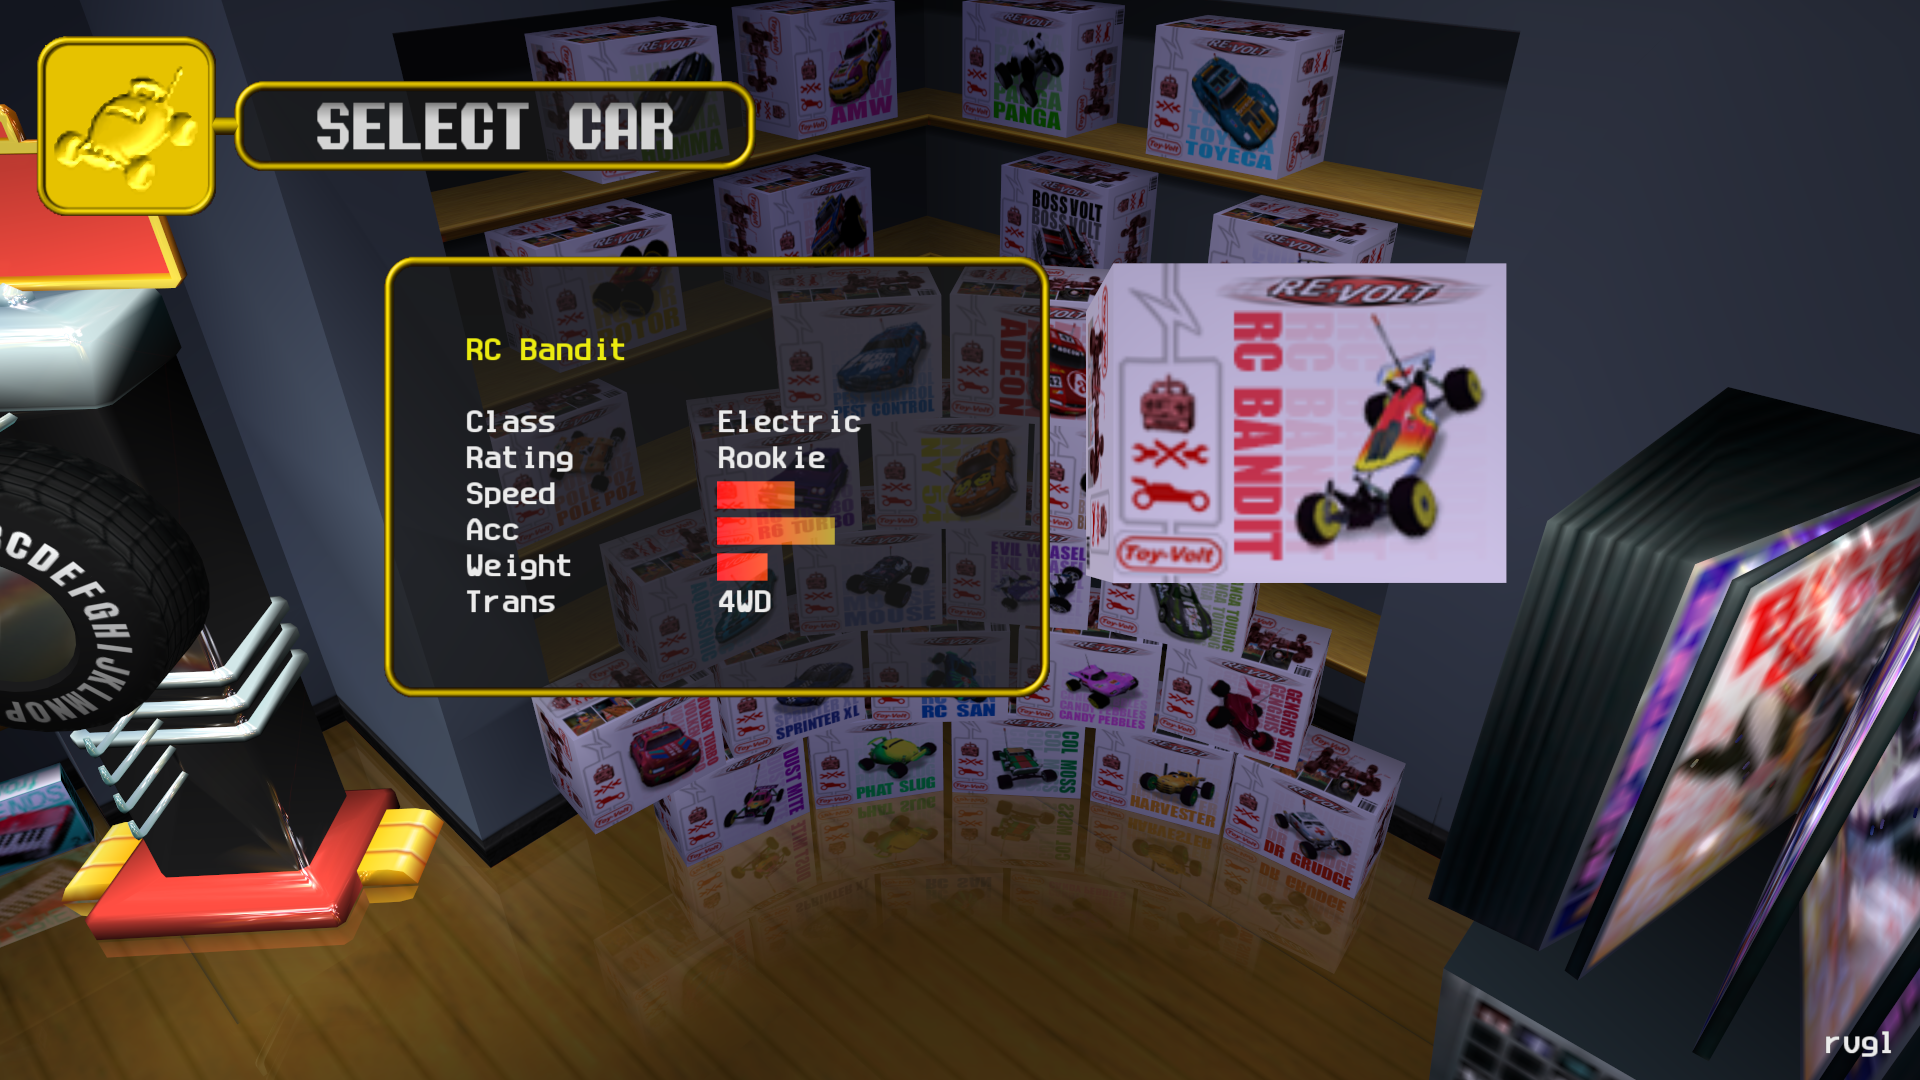
\includegraphics[width=15cm, height=8cm]{img/bandit.png}
  \end{center}
  \caption[Selección de auto en RVGL]{Selección de auto en RVGL}
  \label{fig:bandit}
\end{figure}

De manera habitual, el anfitrión define una categoría de auto con la cual se jugará la sesión. De esta forma, todos los jugadores que se conecten deberán utilizar autos de la categoría definida.

Teniendo en cuenta lo anterior, las sesiones suelen ser nombradas a partir de su categoría asociada. Por ejemplo, si para una sesión se decide jugar autos de la categoría ''Pro'', es normal que esta sea titulada  ''Pros Session'', o ''Pro Races'' al momento de ser anunciada.

\subsubsection{Sala de Espera}
Una vez que el usuario elige su auto, este es llevado a la sala de espera, la cual viene representada por la figura \autoref{fig:lobby}

\begin{figure}[H]
  \begin{center}
    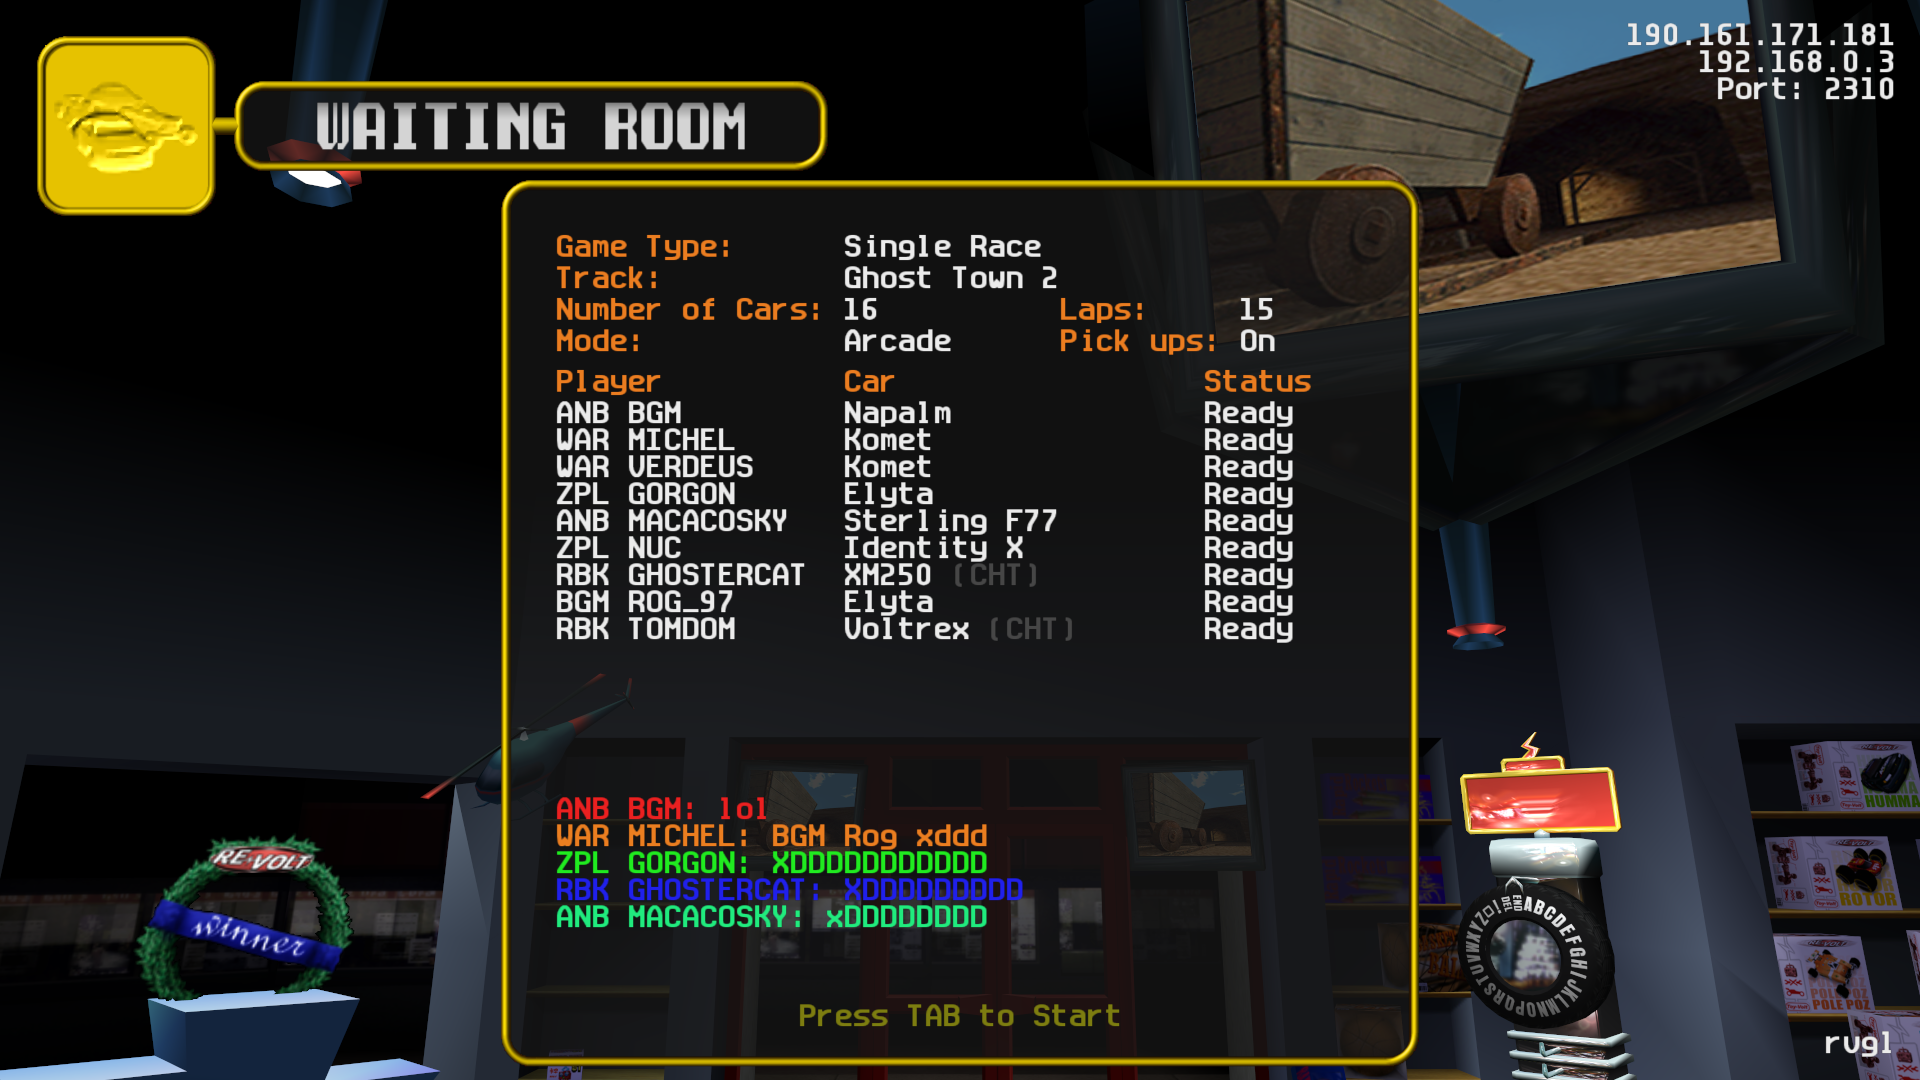
\includegraphics[width=15cm, height=8cm]{img/lobby.png}
  \end{center}
  \caption[Sala de espera en RVGL]{Sala de espera en RVGL}
  \label{fig:lobby}
\end{figure}

Una vez llegados a este punto, sólo se debe esperar a que el anfitrión de la sesión de inicio a las carreras.

\subsubsection{Carreras en Línea}
Normalmente, en las partidas multijugador, suelen jugarse muchas carreras de manera consecutiva. A estas series de partidas en línea se les conoce como ''sesiones''. Cada sesión de Re-Volt consiste en una cantidad predefinida de carreras en pistas determinadas y con cierta clase de autos. Estas determinaciones las realiza el anfitrión de la partida, quien las comunica públicamente de manera oportuna para que todos aquellos que deseen participar tengan en cuenta todas las características de la sesión que van a jugar.

Las siguientes dos ilustraciones presentan las instancias clave dentro del juego. En la \autoref{fig:gameplay}, se puede apreciar la perspectiva del jugador al momento de jugar Re-Volt. Luego, en la \autoref{fig:results}, se puede ver la tabla de resultados que se muestra por pantalla a medida que los corredores finalizan la carrera.

\begin{figure}[H]
  \begin{center}
    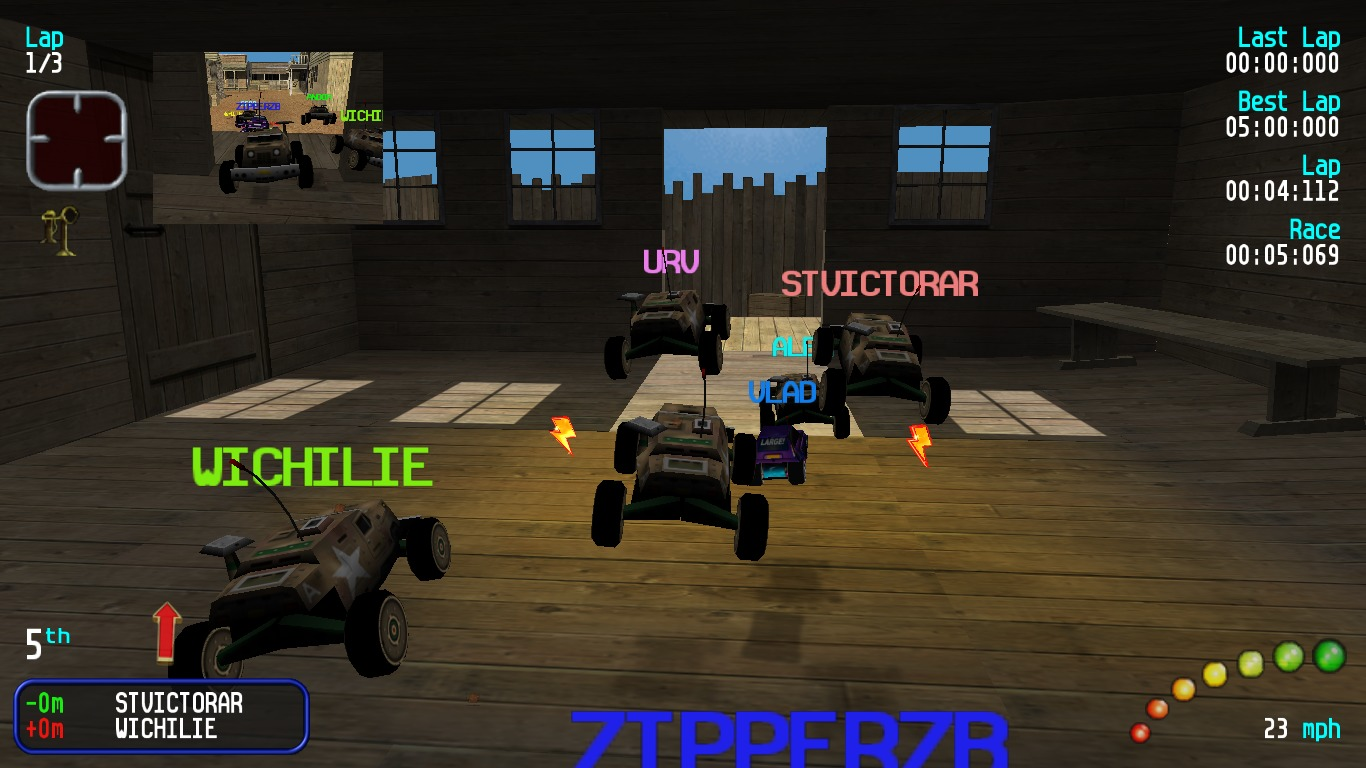
\includegraphics[width=15cm, height=8cm]{img/gameplay.jpg}
  \end{center}
  \caption[Punto de vista del jugador en carrera]{Punto de vista del jugador en carrera}
  \label{fig:gameplay}
\end{figure}

\begin{figure}[H]
  \begin{center}
    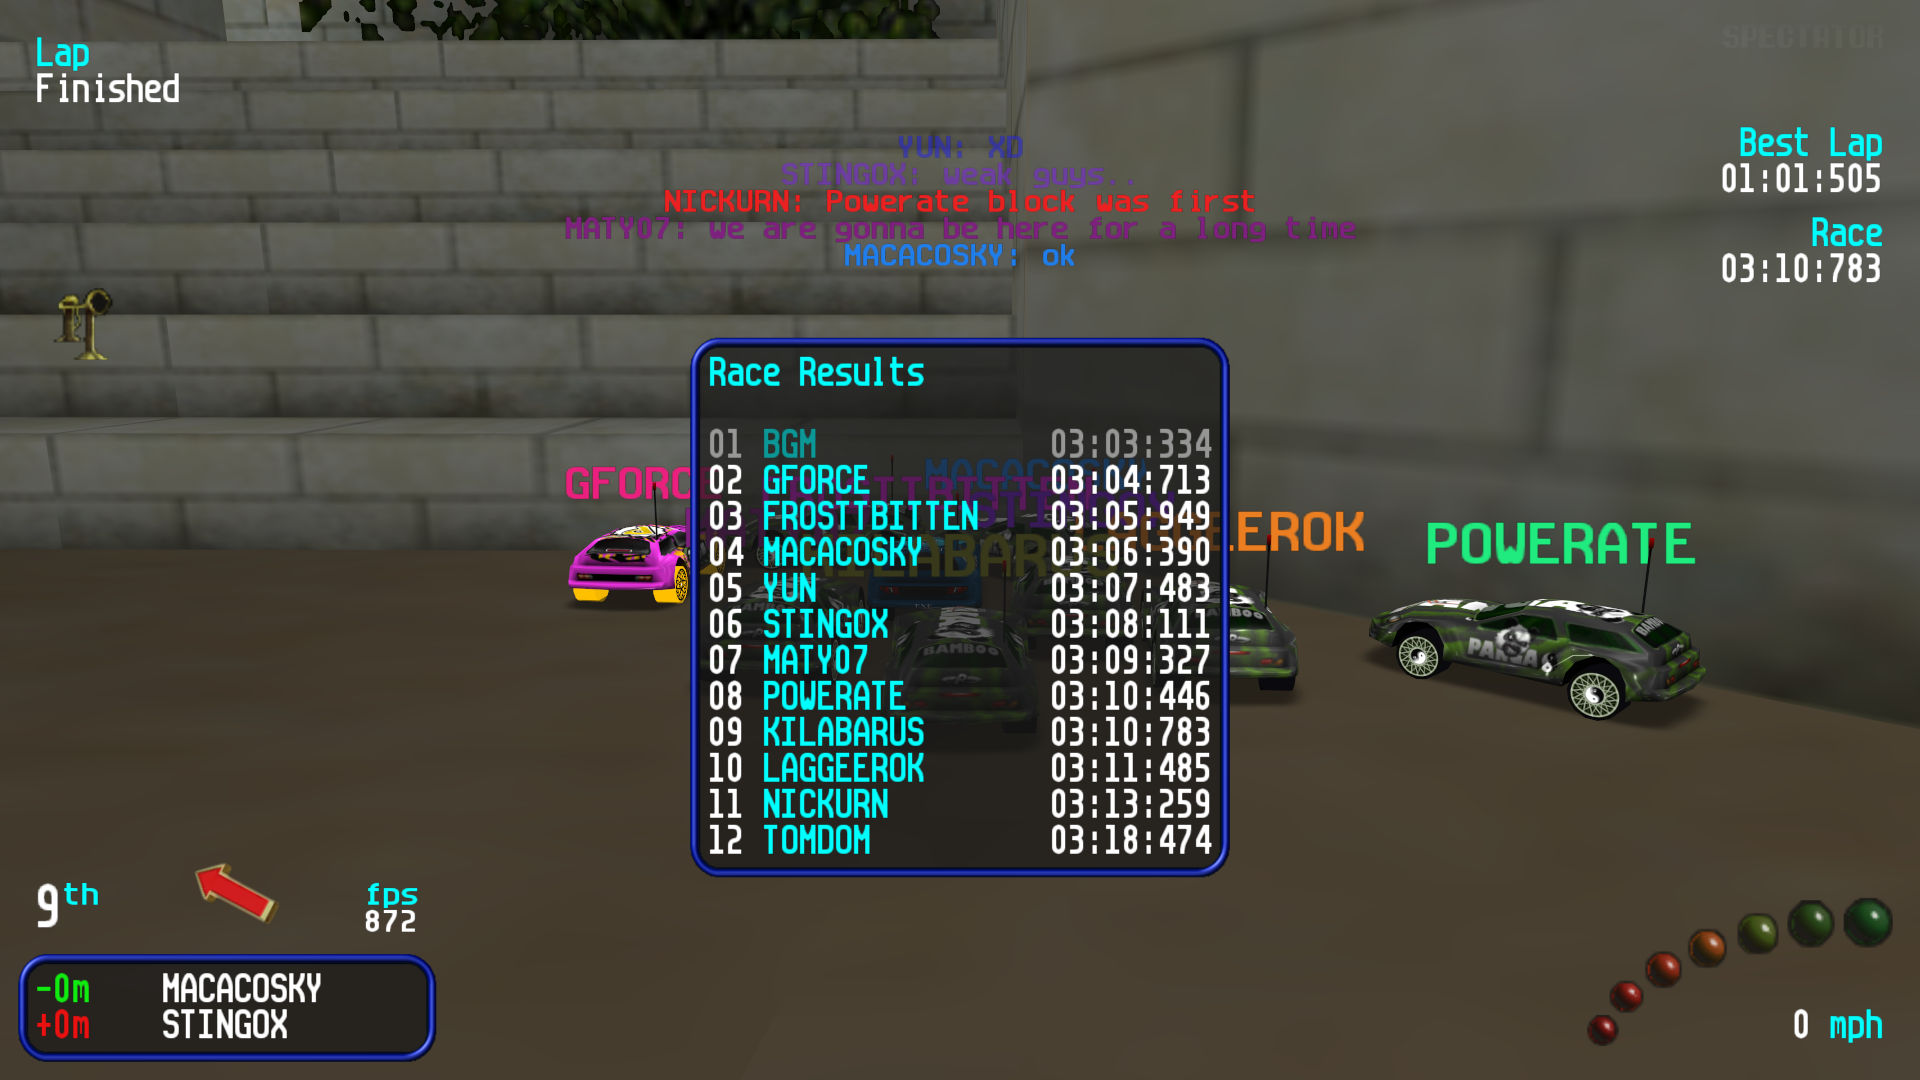
\includegraphics[width=15cm, height=8cm]{img/results.png}
  \end{center}
  \caption[Resultados de carrera en RVGL]{Resultados de carrera en RVGL}
  \label{fig:results}
\end{figure}

\subsection{Re-Volt: OpenGL y los Session Logs}

Para ayudar a llevar una cuenta fiable de todas las carreras jugadas, RVGL introduce una funcionalidad que permite a los jugadores obtener un registro escrito de los resultados de cada carrera. Este registro viene en forma de un archivo separado por comas, el cual es conocido por la comunidad como Session Log. Este es el archivo que utilizan los organizadores y administradores de RVA para calcular los resultados oficiales de las sesiones.

En la \autoref{fig:raw-results}, presentada a continuación, puede apreciarse un extracto del Session Log de una sesión cualquiera, el cual ha sido importado desde Microsoft Excel para una visualización más clara. Este extracto representa una sola de las carreras jugadas en la sesión. Entiéndase que, inmediatamente después de la última línea, vendría escrita la carrera siguiente, y así sucesivamente con todas las demás.

\begin{figure}[H]
  \begin{center}
    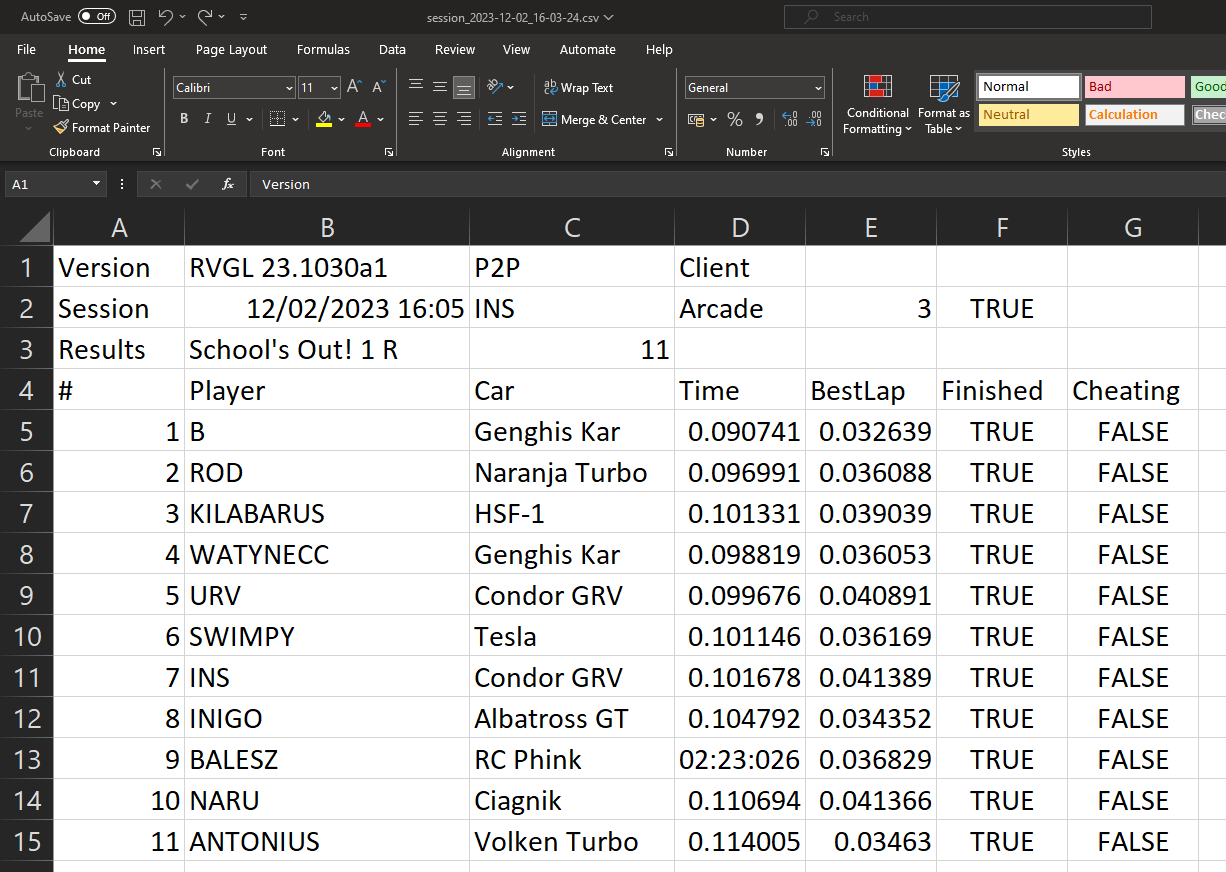
\includegraphics[width=15cm, height=10cm]{raw-results.png}
  \end{center}
  \caption[Session Log de RVGL]{Session Log de RVGL}
  \label{fig:raw-results}
\end{figure}

A continuación, la tabla siguiente es una especificación de los elementos relevantes de un Session Log. Algunos de dichos elementos son utilizados por RVA para calcular los resultados acumulados de las sesiones, para así obtener una tabla con posiciones finales para cada jugador al final de cada sesión.

\begin{center}
	\begin{tabular}{ | l | p{13cm} |}
		\hline
		\multicolumn{2}{|c|}{\textbf{Elementos de un Session Log}} \\
		\hline
		\multicolumn{1}{|c|}{\textbf{Id}} & \multicolumn{1}{|c|}{\textbf{Descripción}} \\
		\hline
		{\textbf{B1}} & Versión de RVGL de la sesión jugada. \\ \hline
		
		{\textbf{C1-D1}} & Protocolo de conexión de la sesión. \\ \hline
		
		{\textbf{B2}} & Fecha y hora de apertura de la sesión. \\ \hline
		
		{\textbf{C2}} & Nombre del jugador anfitrión de la sesión. \\ \hline
		
		{\textbf{D2}} & Tipo de colisión entre autos, seleccionado por el anfitrión. \\ \hline
		
		{\textbf{E2}} & Número de vueltas de esta carrera. \\ \hline
		
		{\textbf{B3}} & Nombre de la pista de esta carrera. \\ \hline
		
		{\textbf{C3}} & Número de jugadores que comenzaron la carrera. Si un jugador se desconecta en mitad de la carrera, este número no se ve afectado. \\ \hline
		
		{\textbf{B5-B15}} & Nombres de los jugadores que participaron de la carrera, agregados de arriba hacia abajo por orden de llegada a la línea de meta. \\ \hline
		
		{\textbf{C5-C15}} & Nombres de los autos utilizados por cada jugador en esta carrera. \\ \hline
		
		{\textbf{D5-D15}} & Tiempo total de la carrera de cada jugador.\\ \hline
		
		{\textbf{E5-E15}} & Mejor vuelta de cada jugador.\\ \hline
		
		{\textbf{F5-F15}} & TRUE si el jugador finalizó la carrera. FALSE si el jugador se desconectó en mitad de la carrera.\\ \hline
		
		{\textbf{G5-G15}} & TRUE si los archivos locales del jugador no corresponden a los archivos del anfitrión. FALSE si estos coinciden. Por ejemplo, ''Cheating'' es TRUE si un jugador modificó localmente la velocidad de su auto.\\ \hline
	\end{tabular}
    \\
\captionof{table}{Tabla de elementos de un Session Log de RVGL}\label{table:sessionlog}
\end{center}

\subsection{Funcionamiento Interno de Re-Volt America}

\subsubsection{Sistema de Temporadas, Rankings y Sesiones}
Históricamente, Re-Volt America se ha dedicado a organizar sesiones multijugador de Re-Volt para su público, así como también se ha preocupado de llevar la cuenta de los resultados de cada carrera que se ha jugado en ellas. Esto lo hace mediante un sistema de temporadas.

Todos los jugadores que, en algún momento u otro, han participado en las sesiones online organizadas por Re-Volt America, han sido indexados en la base de datos de jugadores que mantiene la comunidad. De esta forma, sus victorias, puntos y otras estadísticas asociadas han sido preservadas a lo largo del tiempo.

Para conseguir un sistema atractivo para sus jugadores, Re-Volt America organiza sus sesiones en una serie de rankings, los cuales consisten en 28 sesiones multijugador cada uno, jugandose una sesión al día. Al cumplirse 6 de estos rankings, se completa lo que en RVA se conoce como una temporada.

Cada sesión organizada por RVA consiste en 20 carreras, las cuales se juegan en 20 pistas diferentes. Es por esto que, en una sesión, se producen 20 sets de resultados (1 por carrera).

Cada año, en promedio, se inician dos temporadas, y cada una es nombrada en base a su año de inicio, y su periodo en relación a otras temporadas. Por ejemplo, si en el año 2023 se da inicio a una temporada en el mes de enero, esta vendría a llamarse ''2023'', ya que terminará dentro del mismo año en el que inició. Por otra parte, si la temporada inicia en el mes de diciembre de 2023, esto quiere decir que terminará dentro del año 2024, por lo que pasaría a llamarse ''2023-24''.

Es así como Re-Volt America, desde el año 2017, hasta el presente, ha conseguido consolidarse como la comunidad de Re-Volt predilecta para los jugadores tanto de norteamerica como América latina.

\subsubsection{Paquete de Contenido de RVA}
\label{problem:context:rva:pack}
Re-Volt America cuenta con un paquete de contenido extra para RVGL, el cual es construido por sus administradores y organizadores al principio de cada temporada.

Este paquete consiste en una selección de autos y pistas para RVGL hechos por la comunidad, los cuales tienen el objetivo de extender el contenido original del juego, y así proveer a los usuarios con una experiencia más enriquecedora y variada al momento de jugar en línea.

El paquete de contenido de RVA, más conocido como RVA Pack, es, técnicamente, un conjunto de archivos correspondientes a los autos y pistas que este busca agregar. Estos archivos son mandatorios para poder participar de las sesiones organizadas por RVA. Esto quiere decir que, para que un usuario pueda entrar a una sesión de RVA, este debe tener instalado el RVA Pack en su instalación de RVGL local.

\subsubsection{Sistema de Puntuación}
Como se ha aludido a lo largo del estudio del problema, la comunidad de Re-Volt America cuenta con su propio sistema de puntuación, el cual le sirve para generar estadísticas por jugador, tablas de resultados al final de cada sesión, y demás métricas que, finalmente, promueven la competitividad y enriquecen la experiencia de los usuarios.

El funcionamiento de dicho sistema de puntuación es el siguiente: dependiendo de la posición da cada jugador, al final de cada carrera, a estos se les asigna un puntaje. El mapeo de puntos para una carrera con menos de 10 participantes viene definido por la siguiente función que relaciona posiciones con puntos, respectivamente:

\newpage

\[\hspace*{1.2cm} pos \hspace*{0.3cm} f_1(pos)\]
\[
\mathlarger{
	f_1= 
	\begin{cases}
		1 \to 15 \\
		2 \to 12 \\
		3 \to 10 \\
		4 \to 7 \\
		5 \to 5 \\
		6 \to 4 \\
		7 \to 2 \\
		8 \to 2 \\
		9 \to 1
	\end{cases}
}
\]

Por otro lado, en caso de que la carrera cuente con 10 jugadores o más, el mapeo de puntos sería el siguiente:

\[\hspace*{1.2cm} pos \hspace*{0.3cm} f_2(pos)\]
\[
\mathlarger{
	f_2= 
	\begin{cases}
		1 \to 20 \\
		2 \to 16 \\
		3 \to 12 \\
		4 \to 10 \\
		5 \to 8 \\
		6 \to 8 \\
		7 \to 6 \\
		8 \to 4 \\
		9 \to 2 \\
		10 \to 2 \\
		11 \to 1 \\
		12 \to 1 \\
		13 \to 1 \\
		14 \to 1 \\
		15 \to 1 \\
		16 \to 1
	\end{cases}
}
\]

Por lo tanto, el conjunto que define los posibles puntajes obtenibles viene definido de la siguiente manera:

\[
\mathlarger{
	P = \{1, 2, 4, 5, 6, 7, 8, 10, 12, 15, 16, 20\}
}
\]

Si se tiene que ''\textit{n}'' es la cantidad de jugadores que participaron de una carrera, entonces:

\[
\mathlarger{
	A = \{1, \dots, n\} \subset \mathbb{N}
}
\]

\[
\mathlarger{
	n = \lvert A \rvert
}
\]

Teniendo en cuenta lo anterior, es posible definir una función que, al recibir una posición final de un jugador en una carrera determinada, retorne la cantidad de puntos correspondientes a dicha posición. Esta función vendría definida a continuación, en donde ''\textit{pos}'' es la posición final del jugador en la carrera en cuestión.

\[
\mathlarger{
f : pos \in A \to 
\begin{cases}
	f_1(pos) & \text{if } n < 10\\
	f_2(pos) & \text{if } n \geq 10
\end{cases}
\in P
}
\]

Al finalizar una sesión, los puntajes de cada jugador en cada carrera se suman, lo que entrega un total de puntos por jugador. Una vez sumados, los puntajes finales son normalizados, y sometidos a diferentes procesos de ajuste propios del sistema de RVA. Una vez ajustados, estos pasan a ser los puntajes finales de la sesión de cada jugador.

\subsubsection{Cálculo de Resultados}
Una vez procesados, los resultados son llevados a una tabla final, tal como se puede apreciar en la \autoref{fig:old-results}.

\begin{figure}[H]
  \begin{center}
    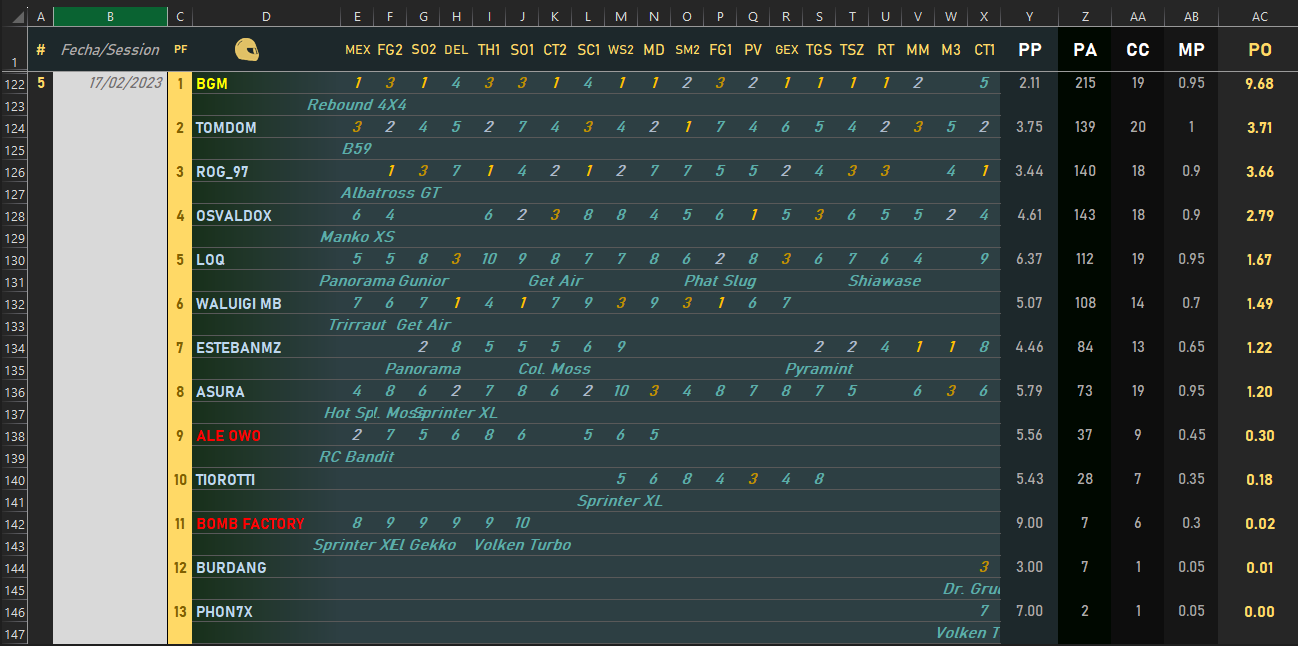
\includegraphics[width=16cm, height=10cm]{old-results.png}
  \end{center}
  \caption[Tabla de resultados de RVA]{Tabla de resultados de RVA}
  \label{fig:old-results}
\end{figure}

\begin{center}
	\begin{tabular}{ | p{5cm} | l | p{7cm} |}
		\hline
		\multicolumn{3}{|c|}{\textbf{Parámetros}} \\
		\hline
		\multicolumn{1}{|c|}{\textbf{Nombre}} & \multicolumn{1}{|c|}{\textbf{Abreviación}} & \multicolumn{1}{|c|}{\textbf{Descripción}} \\
		\hline
		{\textbf{Posición Promedio}} & PP & La suma de las posiciones del jugador, dividida por su cantidad de carreras corridas. \\ \hline
		{\textbf{Puntaje Acumulado}} & PA & La suma total de los puntos correspondientes a las posiciones obtenidas por el jugador. \\ \hline
		{\textbf{Carreras Corridas}} & CC & La cantidad de carreras corridas por el jugador. \\ \hline
		{\textbf{Multiplicador por Participación}} & MP & La cantidad de carreras corridas por el jugador, divida por la cantidad de carreras totales de la sesión. \\ \hline
		{\textbf{Puntaje Oficial}} & PO & El puntaje acumulado del jugador, multiplicado por un factor normalizador de 0.1. \\ \hline
	\end{tabular}
  \\
  \captionof{table}{Tabla de parámetros de RVA}\label{table:parameters}
\end{center}

De acuerdo con la tabla anterior, los cálculos de PA, PP y MP pueden ser representados utilizando las siguientes fórmulas, respectivamente, en donde ''\textit{pos}'' es la posición del jugador en cada carrera, y ''\textit{tot}'' la cantidad total de carreras de la sesión.

\[
\mathlarger{{PA} = \sum_{i=1}^{CC}x=x+f(pos_i)}
\]

\[
\mathlarger{{PP} = \frac{\left(\sum\limits_{i=1}^{CC}x=x+pos_i\right)}{CC}}
\]

\[
\mathlarger{{MP} = \frac{CC}{tot}}
\]

A partir de estos parámetros, podemos calcular el puntaje oficial, o PO, obtenido por el jugador en la sesión en cuestión.

\[
\mathlarger{{PO} = \left(\frac{PA}{PP} \cdot MP\right) \cdot 0.1}
\]

\subsubsection{Multiplicadores por Auto}
Como ya se mencionó anteriormente, al principio de cada temporada, se agregan y se eliminan autos del pack de RVA. Asimismo, RVA introduce el concepto de multiplicadores para dichos autos por temporada.

De acuerdo con el sistema de RVA, el puntaje obtenido por un jugador al finalizar una carrera es alterado por el multiplicador del auto que utiliza en dicha carrera. De esta forma, el puntaje obtenido por el jugador incrementa o disminuye dependiendo del multiplicador asociado a su auto.

Los multiplicadores de cada auto son un reflejo de su potencial para desempeñarse en carreras en línea en comparación a los demás autos de su categoría. Por ejemplo, si un auto es increíblemente rápido, fácil de manejar y no tiene dificultad alguna, entonces a este se le asocia con un multiplicador bajo, para así nivelar los puntos que, potencialmente, pueda obtener un jugador al utilizarlo. Por el contrario, si un auto es muy lento, difícil de manejar, y simplemente es peor que los demás autos de su categoría, entonces se le asocia con un multiplicador alto, para así otorgar puntos extra a quien lo utilice.

La decisión de qué autos son buenos y qué autos son malos, en comparación con los demás de su categoría, es tomada por la administración de RVA en base a pruebas de manejo para los autos, y la experiencia previa en temporadas anteriores. A partir de esta decisión, se le otorga un multiplicador a cada auto.

Considerando los distintos multiplicadores que puede tener cada auto, la fórmula para el cálculo del PA es modificada ligeramente, en donde ''\textit{mul}'' es el multiplicador del auto asociado.

\[
\mathlarger{{PA} = \sum_{i=1}^{CC}x=x+f(pos_i) \cdot mul_i}
\]

Como se explicó anteriormente, existen varias categorías de autos en Re-Volt. Si bien las sesiones de RVA corresponden a una categoría a la vez, el sistema admite que jugadores elijan autos hasta 3 clases por debajo de la categoría de la sesión. Por ejemplo, si la sesión es publicada como de categoría ''Pro'', un jugador puede elegir un auto de categoría ''Semi-Pro''.

De acuerdo con el sistema de RVA, por cada categoría de diferencia entre la sesión y el auto elegido por el jugador, a este se le otorga un bono de 0.25, el cual se adiciona al multiplicador de su auto. Si en el ejemplo anterior la sesión era ''Pro'' y el auto ''Semi-Pro'', entonces al multiplicador del auto se le suma directamente 0.25. Si la diferencia fuese de 2 categorías, entonces se le sumaría 0.5.

Teniendo en cuenta lo anterior, la fórmula es modificada nuevamente. En este caso, la variable ''\textit{delta}'' representa el bono asignado al jugador en la carrera.

\[
\mathlarger{{PA} = \sum_{i=1}^{CC}x=x+f(pos_i) \cdot \left(mul_i + delta_i\right)}
\]

\section{Sistema Actual}

\section{Problemática Actual}
Hoy en día,  RVA utiliza una aplicación llamada ''RVA-Points'', la cual está hecha exclusivamente para procesar los Session Logs generados por RVGL y transformarlos en archivos separados por comas que contienen los resultados de las sesiones en el formato de RVA.

Una vez procesados los Session Logs, RVA lleva la cuenta de sus temporadas y jugadores utilizando Microsoft Excel como una pseudo base de datos para registrarlos, y Dropbox para la sincronización de archivos entre administradores.

Cada temporada, los administradores manejan un documento maestro de Excel, el cual, en resumidas cuentas, es utilizado para registrar los resultados de cada sesión y, a la vez, llevar la cuenta de los puntos por jugador. Esto se consigue utilizando macros y demás componentes característicos de Excel.

Los documentos relacionados a cada temporada son archivados utilizando una carpeta compartida en Dropbox.

Actualmente, el proceso diario para calcular y publicar los resultados de cada sesión es llevado a cabo, de manera semiautomática, por los administradores de RVA. Este proceso consiste en los siguientes pasos:

\begin{enumerate}
	\item Una vez finalizada la sesión, se busca el Session Log generado por RVGL, y este llega a los administradores de RVA.
	\item Se revisan los nombres de usuario manualmente. Esto se hace en caso de que algún jugador haya utilizado un nombre ligeramente distinto al que usa normalmente.
	\item El Session Log de la sesión es importado desde ''RVA-Points''. Este programa procesa el Session Log, y lo transforma en resultados ordenados en el formato de RVA.
	\item También desde ''RVA-Points'', los resultados procesados son exportados a otro archivo separado por comas.
	\item Se copian los contenidos del archivo exportado al documento maestro de la temporada actual.
	\item Se agrega cierta información de manera manual, como la fecha y número de la sesión.
	\item Se revisa manualmente que los nombres de usuario de la sesión correspondan a los nombres que ya figuran en el documento maestro.
	\item Se publica una fotografía de la tabla de resultados de la sesión en el Discord de RVA.
	\item Se publica una fotografía del ranking actualizado con los datos de la sesión en el Discord de RVA.
\end{enumerate}

A raíz de este largo y tedioso proceso de cálculo y manejo de resultados, se ha dado origen a este proyecto de título, como una oportunidad de mejorar dicho proceso, y poder ofrecer así una mejor experiencia de usuario tanto para los jugadores de RVA, como para los organizadores de la comunidad, quienes dedican su tiempo y esfuerzo a mantener estos registros históricos al día para todos.

\subsection{Diagrama de la Situación en la Actualidad}
Teniendo en cuenta el contexto del problema, la situación en la actualidad puede representarse a través del siguiente diagrama BPMN:

\begin{figure}[H]
  \begin{center}
    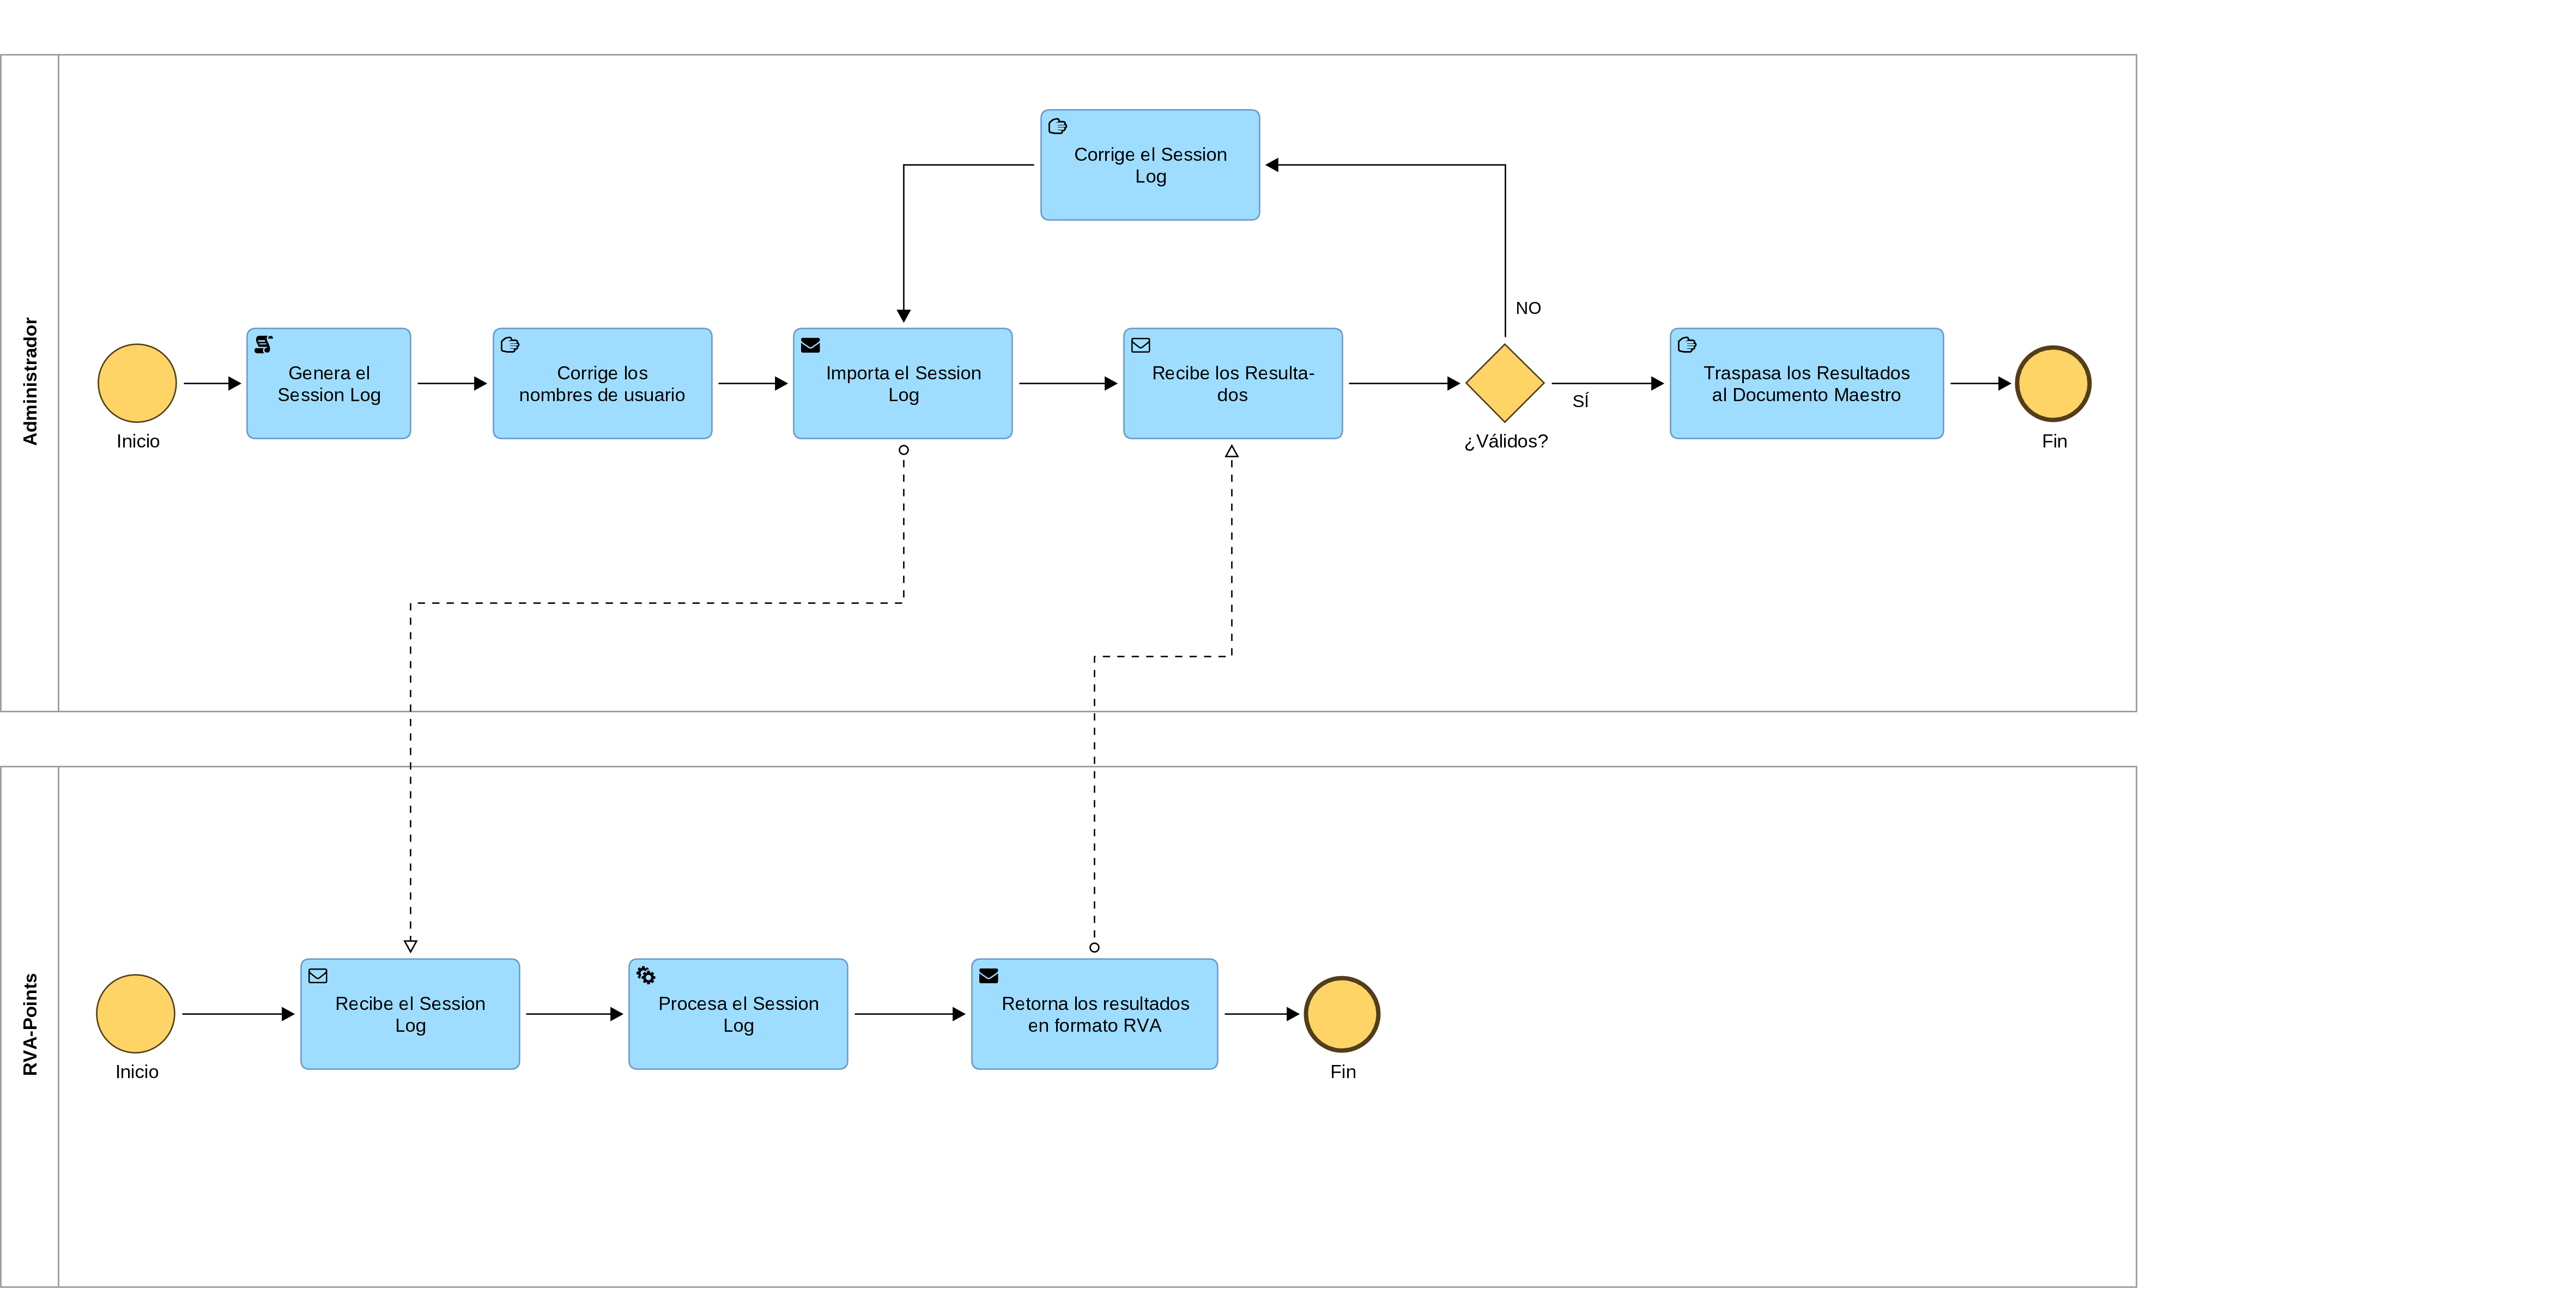
\includegraphics[width=18.5cm, height=10cm]{bpmn1.png}
  \end{center}
  \caption[Diagrama BPMN del proceso actual de cálculo de puntos]{Diagrama BPMN del proceso actual de cálculo de puntos}
  \label{fig:bpmn}
\end{figure}

\section{Propuesta de Solución}
Para poder solucionar los desafíos y problemas que enfrenta la comunidad de Re-Volt America hoy en día, se propone desarrollar una plataforma web que integre todo el proceso de cálculo de puntos por sesión, así como también el manejo de estadísticas individuales por jugador.

La aplicación web será desarrollada utilizando el framework para desarrollo de aplicaciones full-stack ''Ruby on Rails''. La persistencia de datos se implementará a través de MongoDB, y se utilizará Redis encima de todo lo anterior para implementar un caché de información pesada, tal como los cálculos complejos que se necesitan servir al usuario con gran frecuencia.

Los principales usuarios del sistema propuesto serían los administradores de RVA y los jugadores de la comunidad (usuarios sin privilegios de ningún tipo). Asimismo, también existirán usuarios con roles específicos equivalentes a los roles que existen dentro de RVA, los cuales son ''organizador'' y ''moderador''. Los administradores, organizadores y moderadores son lo que se conoce como el staff de RVA.

Todo lo descrito en los párrafos anteriores será detallado de manera oportuna a lo largo del resto de este informe.

\section{Soluciones Similares Disponibles}
A continuación, se describen las soluciones disponibles que pueden ser catalogadas como similares al proyecto que se presenta.

\subsection{Aplicación para Cálculo de Puntos de Re-Volt I/O}
Existe un trabajo similar hace varios años, el cual fue desarrollado por la comunidad europea de RVGL: Re-Volt I/O.

Este trabajo se trata de una aplicación web que permite a los administradores de Re-Volt I/O importar los resultados de las sesiones multijugador, y poder visualizarlos dentro de la misma página; sin embargo, dicho proyecto no cuenta con ningún tipo de interconexión entre resultados, lo que quiere decir que cada sesión de carreras publicada en dicho sitio es independiente de otras. Debido a lo anterior, este proyecto no cuenta con perfiles de usuario, y por ende no permite visualizar estadísticas de ningún tipo, ni tampoco relacionar tablas de resultados entre si.

En general, esta solución fue concebida para ser algo simple y rápido que sirviera para calcular y renderizar resultados de manera oportuna, y no con una visión de persistencia en mente. A continuación, en la \autoref{fig:io-results}, puede apreciarse la tabla de resultados generada por la aplicación web de Re-Volt: I/O.

\begin{figure}[H]
  \begin{center}
    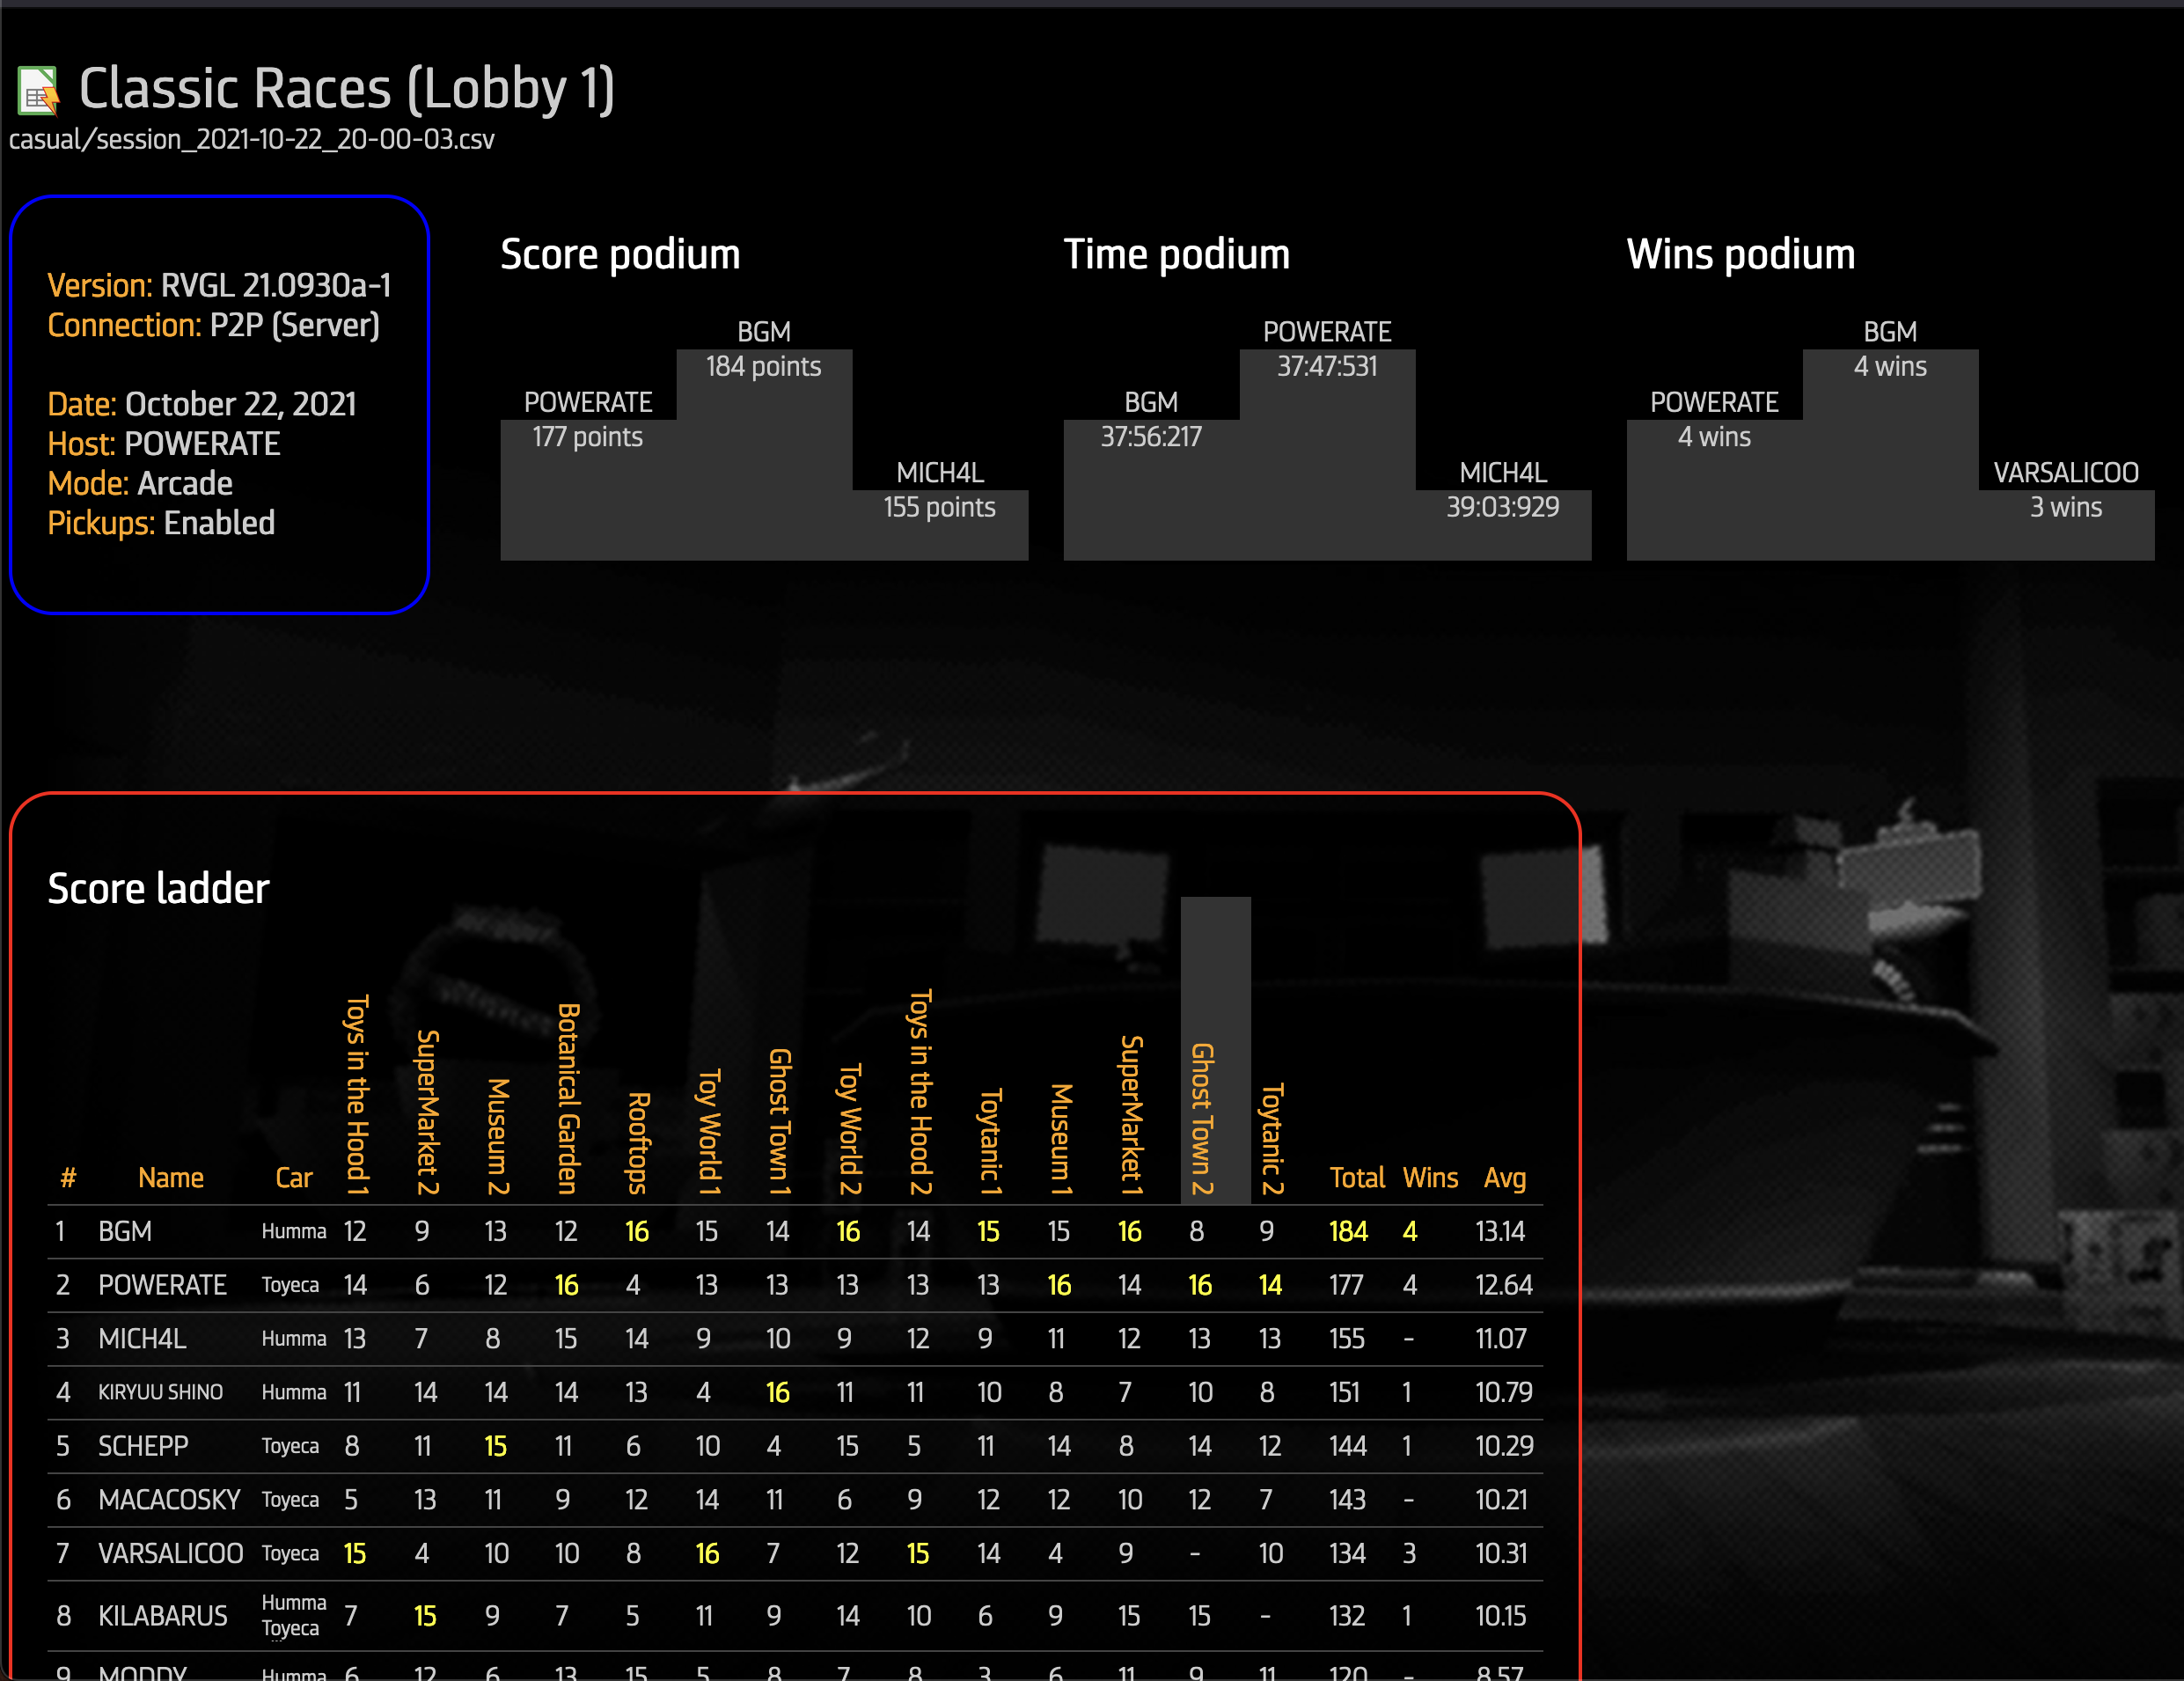
\includegraphics[width=15.5cm, height=15cm]{io-results.png}
  \end{center}
  \caption[Software de cálculo de resultados de Re-Volt: I/O]{Software de cálculo de resultados de Re-Volt: I/O}
  \label{fig:io-results}
\end{figure}

\section{Justificación del Problema}
Actualmente, no existe ninguna plataforma que permita a los usuarios registrarse o visualizar resultados y estadísticas de las sesiones multijugador organizadas por la comunidad. Lo anterior significa que, cuando se juegan partidas online, no es posible obtener de manera automática rankings, estadísticas por vehículo y menos por usuario, ya que no hay forma de vincular, de manera definitiva, a los jugadores a través de un perfil dentro del juego. Es por ello que un usuario de nuestra comunidad no puede saber cuántas carreras o sesiones ha ganado con cierto auto, o en cierta pista, cómo se compara al resto, qué porcentaje de carreras ha perdido, ganado, etc.
